
\documentclass[10 pt]{article}  



%% Includes %%%%%%%%%%%%%%%%%%%%%%%%%%%%%%%%%%%%%%%%%%%%%%%%%%%%%%%%%%%%%%%%%%%%%%%%%%%%%%
\usepackage[natbib=true,style=numeric-comp,sorting=none,firstinits=true,maxbibnames=99]{biblatex}
\usepackage{times}
\usepackage{multicol}
\usepackage[bookmarks=true]{hyperref}
\usepackage{graphicx} % for pdf, bitmapped graphics files
\usepackage{booktabs} % fancy tables
\usepackage{subfig} % self explanatory
\usepackage{amsmath, amsfonts}
\usepackage{amssymb}
\usepackage{float}
\usepackage{dblfloatfix}    % To enable figures at the bottom of page
\usepackage{flushend} % Equalize last two ref cols

\usepackage[svgnames]{xcolor}
\usepackage{listings}

\newcommand{\diag}{\mathop{\mathrm{diag}}}

\definecolor{dkgreen}{rgb}{0,0.6,0}
\definecolor{gray}{rgb}{0.5,0.5,0.5}
\definecolor{mauve}{rgb}{0.58,0,0.82}

\lstset{language=Python,
    basicstyle=\small\ttfamily,
    stringstyle=\color{DarkGreen},
    otherkeywords={0,1,2,3,4,5,6,7,8,9},
    morekeywords={TRUE,FALSE},
    deletekeywords={data,frame,length,as,character},
    keywordstyle=\color{blue},
    commentstyle=\color{DarkGreen},
}

%%%%%%%%%%%%%%%%%%%%%%%%%%%%%%%%%%%%%%%%%%%%%%%%%%%%%%%%%%%%%%%%%%%%%%%%%%%%%
\graphicspath{ {figs/} }

%\addbibresource{library.bib}

\begin{document}

\title{ \LARGE \bf Implementing an MNIST Variational Autoencoder in TensorFlow}

\author{Nate Merrill}

\maketitle

The MNIST hand-written digits dataset is by far the most famous computer vision
dataset available. In this tutorial, we will step through how to create a simple 
variational autoencoder for this data using the TensorFlow library in python.

The first step is to import the necessary modules. For this script we 
will need \texttt{tensorflow}, \texttt{numpy}, and \texttt{matplotlib.pyplot}.

\begin{lstlisting}
import tensorflow as tf
import numpy as np
from matplotlib import pyplot as plt
mnist = tf.keras.datasets.mnist
\end{lstlisting}

Next we need to define the class for our model.
We are encoding the input images into a latent space of dimension 2 so that we can visualize the results.
In this script, I opted to use three four fully-connected layers to decrease the input dimension to
4, which is then sliced in half to make our two latent variables, 
$\boldsymbol{\mu}$ and $\boldsymbol{\sigma}$. 
The latent variables are trained to parameterize a Gaussian distribution $\mathcal{N}(\boldsymbol{\mu}, \diag(\exp(\boldsymbol{\sigma})))$.
In this implementation, $\boldsymbol{\sigma}$ is the natural logarithm of the variance for our distribution.
The latent variables are optimized to construct a standard normal distribution via the Kullback-Leibler Divergence:
\begin{align}
    \mathcal{D}[\mathcal{N}(\boldsymbol{\mu}, \diag(\exp(\boldsymbol{\sigma})))\ ||\ 
    \mathcal{N}(\mathbf{0}, \mathbf{I})] = \notag\ \ & \\
    \frac{1}{2}((\sum_i \exp(\sigma_i) - \sigma_i + \boldsymbol{\mu}^\intercal\boldsymbol{\mu}& - 
    \dim(\boldsymbol{\mu})) 
\end{align}

With the latent variables, we can now construct the input to the decoder.
$\boldsymbol{\epsilon}$ is sampled from a standard normal distribution, and the latent variable $\mathbf{z} = \boldsymbol{\mu} + diag(exp(\boldsymbol \sigma))^{\frac{1}{2}}\boldsymbol{\epsilon}$ is defined.
%
$\mathbf{z}$ is equivalent to sampling our constructed distribution, but, since sampling
is nondifferentiable, we have to resort to what is called the ``resampling technique'' which
uses a sampled standard normal random variable to perform an operation that is equivalent to 
sampling our distribution, but differentiable.

$\mathbf{z}$ is then fed into the decoder, which uses fully connected layers to upscale
up to the original image resolution.
The output of the decoder is then sent to the reconstruction loss:
\begin{equation}
    -\sum_{h, w, c}x_{h,w,c} \log(r_{h,w,c}) + (1 - x_{h,w,c}) \log(1-r_{h,w,c})
\end{equation}
%


\begin{lstlisting}
class VAE:
    def __init__(self, epochs=5, batch_sz=16):
        """Constructor"""

        # Input data Tensor
        self.x = tf.placeholder(tf.float32, shape=[None, 28**2]) 
        fc = self.x
        for n in [256, 128, 64]:
            fc = tf.layers.dense(fc, units=n,
                    activation=tf.nn.elu)
        fc = tf.layers.dense(fc, units=4,
                activation=None)
        
        mu = fc[:,:2]

        # estimate log sigma^2 for numerical stability
        log_sig_sq = fc[:,2:]

        # z = mu + sigma * epsilon
        # epsilon is a sample from a N(0, 1) distribution
        eps = tf.random_normal(tf.shape(mu), 0.0, 1.0, dtype=tf.float32)

        # Random normal variable for decoder :D
        self.z = tf.add(mu, tf.sqrt(tf.exp(log_sig_sq)) * eps, name='z')
        fc = self.z
        for n in [256, 128, 64]:
            fc = tf.layers.dense(fc, units=n,
                    activation=tf.nn.elu)
        fc = tf.layers.dense(fc, units=4,
                activation=None)
        
        # sigmoid bounds answer to [0,1] for images
        rec = tf.layers.dense(fc, units=28**2,
                activation=tf.sigmoid)
        self.rec = rec
        # reconstruction loss
        self.rec_loss = tf.reduce_mean(
                      -tf.reduce_sum(self.x * tf.log(tf.clip_by_value(rec, 1e-10, 1.0))
                      + (1.0 - self.x) * tf.log(tf.clip_by_value(1.0 - rec, 1e-10, 1.0)),
                      axis=1))

        # stdev is the diagonal of the covariance matrix
        # KLD( (mu, sigma) , N(0,1) ) = .5 (tr(sigma2) + mu^T mu - k - log det(sigma2))

        self.kld = tf.reduce_mean(
                   -0.5 * (tf.reduce_sum(1.0 + log_sig_sq - tf.square(mu)
                   - tf.exp(log_sig_sq), axis=1)))

        self.loss = self.kld + self.rec_loss
        self.opt = tf.train.AdamOptimizer().minimize(self.loss)

    def step(self, batch, sess):
        kld, rec_loss, _ = sess.run([self.kld, self.rec_loss, self.opt],
                            feed_dict={self.x: batch})
        return kld, rec_loss
\end{lstlisting}

After we train the network, we wish to visualize the results. 
This function will create a grid over [-2,2] in each direction and evaluate 
the decoder at each 2D location. 
We will see later that the autoencoder disributes each type of digit well throughout
the latent space.

\begin{lstlisting}
def display_manifold(model, sess):
    # display a 30x30 2D manifold of digits
    n = 30
    figure = np.zeros((28 * n, 28 * n))
    # linearly spaced coordinates corresponding to the 2D plot
    # of digit classes in the latent space
    grid_x = np.linspace(-2, 2, n)
    grid_y = np.linspace(-2, 2, n)[::-1]

    for i, yi in enumerate(grid_y):
        for j, xi in enumerate(grid_x):
            z_sample = np.array([[xi, yi]])
            x_decoded = sess.run(model.rec, 
                    feed_dict={model.z: z_sample})
            digit = x_decoded[0].reshape(28, 28)
            figure[i * 28: (i + 1) * 28,
                   j * 28: (j + 1) * 28] = digit

    plt.figure(figsize=(10, 10))
    start_range = 28 // 2
    end_range = (n - 1) * 28 + start_range + 1
    pixel_range = np.arange(start_range, end_range, 28)
    sample_range_x = np.round(grid_x, 1)
    sample_range_y = np.round(grid_y, 1)
    plt.xticks(pixel_range, sample_range_x)
    plt.yticks(pixel_range, sample_range_y)
    plt.xlabel("z[0]")
    plt.ylabel("z[1]")
    plt.imshow(figure, cmap='Greys_r')
    plt.savefig("latent.png")
    plt.show()

\end{lstlisting}

Finally, we need to load the MNIST data and train the network with random batches.
It is easy to use \texttt{numpy.random.randint} to get random indices for the data
tensor, and just index them directly.
Here I am using a batch size of 256, and training for 5000 iterations.
This should be able to run on a CPU in just a few minutes. 
At the end of training, we can run our \texttt{display\_manifold} function to visualize the results.

\begin{lstlisting}
if __name__ == '__main__':
    
    # ignore testing data and labels
    (x_train, _),_ = mnist.load_data()
    x_train = (x_train / 255.0).reshape(-1, 28**2)

    model = VAE()
    
    batch = 256
    iterations = 5000

    with tf.Session() as sess:
        sess.run(tf.global_variables_initializer())
        for i in range(iterations):
            batch_idx = np.random.randint(len(x_train), size=batch)
            x_batch = x_train[batch_idx, :]
    
            kld, rec_loss = model.step(x_batch, sess)

            if i % 100 == 0:
                print("Iteration%d:KLD=%f,RecLoss=%f" % (i, kld, rec_loss))

        display_manifold(model, sess)

\end{lstlisting}
\vspace{2000pt}
Here you can see what my manifold looks like:
\begin{figure} [H]
    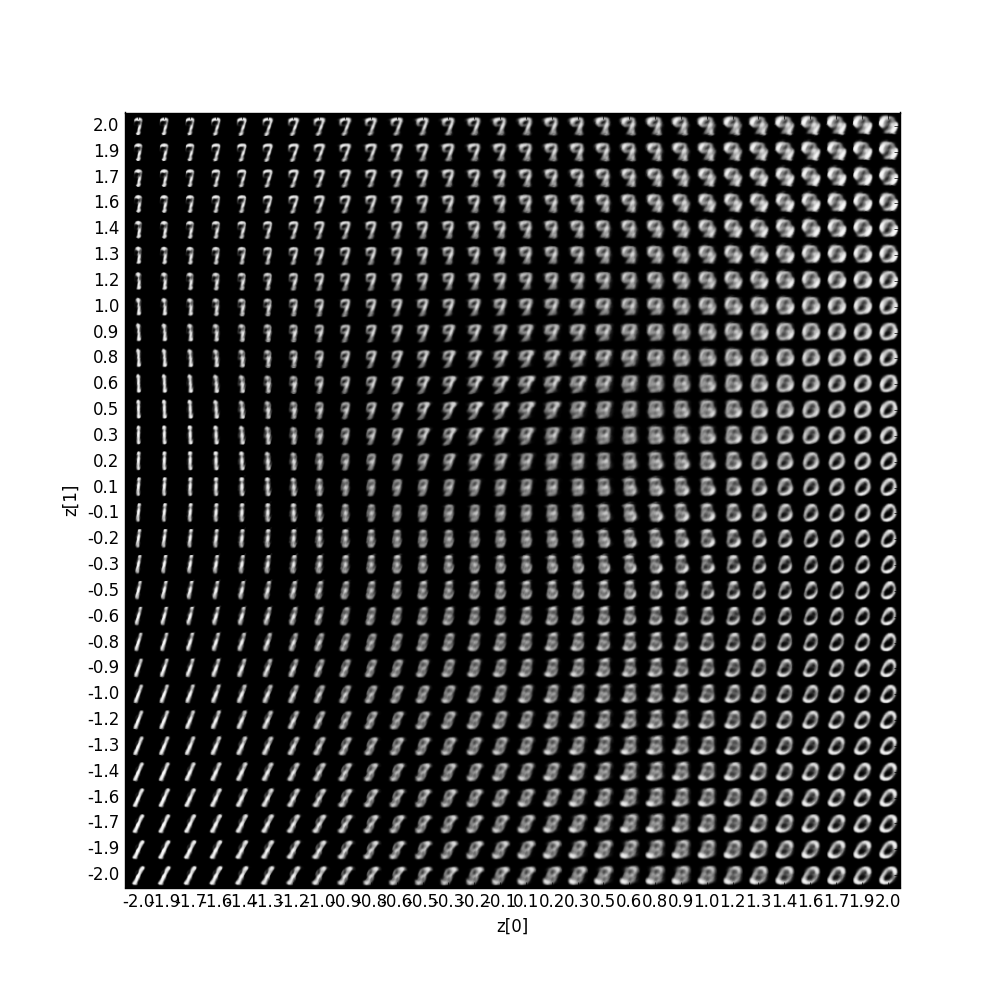
\includegraphics[width=\textwidth]{figs/latent}
\end{figure}

The network is able to encode information about all of the hand-written digits with just 
two degrees of freedom.

%% Bib %%%%%%%%%%%%%%%%%%%%%%%%%%%%%%%%%%%%%%%%%%%
%\printbibliography

%%%%%%%%%%%%%%%%%%%%%%%%%%%%%%%%%%%%%%%%%%%%%
\end{document}
